\documentclass[11pt]{article}

\usepackage{geometry}
\geometry{marginparwidth=1cm,a4paper,verbose,tmargin=1.5cm,bmargin=1.5cm,lmargin=1.5cm,rmargin=1.5cm,headheight=0cm,headsep=0cm,footskip=0cm}
\usepackage{cite}
\setlength\parindent{0pt} % set indent to zero
\setlength{\parskip}{1.2em} % give a bit of space between paragraphs

\bibliographystyle{plain} % citation and bib style
\usepackage{grffile} %for underscores in file names
\usepackage[]{algorithm2e} % for typesetting the riboSeed algorithm
\usepackage{lineno, color} % controls line numbering
% \linenumbers % just in body, not in bibliography or abstract
\modulolinenumbers[5]  % number every 5th line
% format our line numbers, cause no one likes boring numbers
\renewcommand\linenumberfont{\normalfont\tiny\color{blue}}

\usepackage{booktabs}  % less yucky tables
% nice little thing for table spacing (thanks Markus Püschel)
\newcommand{\ra}[1]{\renewcommand{\arraystretch}{#1}}


% my lined-off abstract
\newenvironment{myabstract}{%
\begin{quote} \baselineskip15pt \rule{.89\textwidth}{1.5pt} \vskip .22cm}
{ \vskip .04cm \rule{.89\textwidth}{1.5pt} \end{quote}}



\title{riboSeed: it's whats for dinner}



\author
{Nicholas R Waters,$^{1,2\ast}$ Florence Abram,$^{1}$  Ashleigh Holmes,$^{2}$ Fiona Brennan,$^{1,3}$ and Leighton Pritchard$^{2}$\\
\\
\normalsize{$^{1}$National University of Ireland, Galway}\\
\normalsize{$^{2}$The James Hutton Institute, Dundee, Scotland}\\
\normalsize{$^{3}$Teagasc, Johnstown Castle, Wexford}\\
\\
\small{$^\ast$To whom hate mail should be addressed; E-mail: n.waters4@nuigalway.ie.}
}
\date{}

\usepackage{graphicx}
\graphicspath{ {riboFigs/} }

\begin{document}
\baselineskip22pt  % set line spacing; double spacing is 2xfontsize, in this case 11
\maketitle


\begin{myabstract}
The vast majority of bacterial genome sequencing has been performed using Illumina short reads. Because of the inherent difficulty of resolving repeated regions with short reads alone, only 10\% of sequencing projects have resulted in a closed genome. The most ubiquitous repeated regions are those coding for ribosomal operons (rDNAs), which can occur in a bacterial genome between 1 and 15 times. Here, we show that the genomic context in which rDNAs occur is conserved across taxa. We demonstrate that within a single genome, the regions flanking the rDNAs are unique. By utilizing the conserved nature of rDNAs across taxa and the uniqueness of their flanking regions, targeted pseudocontigs can be generated by iteratively assembling reads mapping to a reference’s rDNAs, and these pseudocontigs can be used to assemble across rDNAs. This method, implemented as riboSeed, reduces the number of contigs in the assembly, and when used in conjunction with other genome polishing tools, can result in closure of a genome.
\end{myabstract}
\begin{linenumbers}


\section*{Background}
\begin{table}[]
\centering
\caption{NCBI Genome Assemblies of Bacteria}
\label{table:completions}
\begin{tabular}{llllll}
  Date              & Total & Complete genome & Chromosome & Scaffold & Contig \\
  \hline
January 4th, 2017 & 85799 & 6255            & 1143       & 39972    & 38429  \\
May 17th, 2017    & 96849 & 7212            & 1254       & 42839    & 43899

\end{tabular}
\end{table}

Sequencing bacterial genomes has become much more cost effective and convenient, but the number of complete, closed bacterial genomes remains a small fraction of the total number sequenced (Table \ref{table:completions}). The length of short reads is increasing, but even with the advent of new long-read technologies, bacterial assembly remains a major bottleneck\cite{Nagarajan2010,Brouwer2016}. Although draft genomes are often of very high quality and suited for many types of analysis, researchers are forced to choose between working with these draft genomes (and the inherent potential loss of data), or spending time and resources polishing the genome with some combination of in silico tools, PCR, optical mapping, resequencing, or hybrid sequencing\cite{Nagarajan2010}. Many in silico genome finishing tools are available, and we summarise several of these in Table \ref{table:tools}.




\begin{table}[]
\centering
\caption{Alternative in silico genome polishing tools}
\label{table:tools}
\resizebox{\textwidth}{!}{
\begin{tabular}{llp{9cm}}
  Tool & Reference & Method Summary \\
  \hline
  Boetzer, et al’s GapFiller & Boetzer2012\cite{Boetzer2012} & utilize paired end and other short read information to close contig junctions \\
  % SOAPdenovo2’s
  GapCloser/IMAGE & Luo2012, Tsai2010\cite{Luo2012, Tsai2010} & iteratively use reads that are mapped to contigs, to close contig junctions \\
  CloG & Yang2011\cite{Yang2011} & use trimmed de novo contigs in hybrid assembly followed by a stitching algorithm \\
  FGap & Piro2014,Guizelini2016\cite{Piro2014,Guizelini2016} & use BLAST to find potential gap closures from alternate assemblies, libraries or references. \\
  GFinisher & Guizelini2016\cite{Guizelini2016} & use GC-skew to refine assemblies \\
  Nadalin, et al’s GapFiller & Nadalin2012\cite{Nadalin2012} & local assembler using a hash-based method to produce “long-reads” from paired end sequencing data, which can then be used in a de novo assembly. \\
  CONTIGuator & Galardini2011\cite{Galardini2011} & use contigs from a de novo assembly along with one or more reference sequences to generate a contig map and PCR primer sets to validate in the lab. \\
  Konnector & Vandervalk2015 \cite{Vandervalk2015} & use paired end reads to make long reads to be used in a Bloom filter representation of a de Bruijn graph \\
  MapRepeat & Mariano2015\cite{Mariano2015} & use a directed scaffolding method to fill in rDNA gaps, but limited to Ion Torrent reads, and affected by inversions between rDNAoperons \cite{Mariano2016} \\
  GRabB & Brankovics2016\cite{Brankovics2016} & Selective assembly tandem rDNA clusters and mitochondria
\end{tabular}
}
\end{table}


The number of Illumina entries in NCBI’s Sequence Read Archive (SRA) \cite{Kodama2012} continues to outnumber all other technologies combined by about an order of magnitude (sup table 3). Draft assemblies from these datasets have systematic problems common to short read datasets, namely gaps in the sequences due to the difficulty of resolving assemblies of repeated regions\cite{Whiteford 2005, Treangen 2013}. Therefore it may be possible to obtain additional sequence information from short read datasets in the SRA, and improve on current assemblies, by improving the ability to resolve assemblies through repeated regions.


The most ubiquitous repeated regions are those coding for ribosomal RNAs. Sequencing of the 16S ribosomal region is widely used to identify bacteria and explore microbial community dynamics\cite{Weisburg1991,Clarridge2004,Woese1990,Case2007}, as the region is conserved within taxa, yet retains enough variability to act as a bacterial “fingerprint” to separate clades informatively. However, the 16S, 23S, and 5S ribosomal subunit coding regions (rDNA) are often present multiple times in a single genome, commonly exhibiting polymorphism \cite{Coenye2003,Moreno2002,Lukjancenko2010, Větrovský2013}. These long, inexactly repeated regions\cite{Agrawal2016, Alkan2011} are problematic for short-read genome assembly. Other large repeated regions also exist, but none as pervasive as rDNAs, as ribosomes are essential for cell function. As rDNAs are frequently used as a sequence marker for taxonomic classification, resolving their genomic context could increase the accuracy of community analysis in cases where polymorphic rDNAs from the same strain result in multiple operational taxonomic units. as ribosomes are essential for cell function.  Although a PCR-based method has been developed\cite{Eastman2015}, no effective in silico method established to resolve the repeats introduced by rDNAs when assembling Illumina data. We present here an in silico method, riboSeed, to capitalize on the genomic conservation of these regions within a taxon, to improve resolution of these normally difficult regions and provide a means to benefit from unexploited information in the SRA.

riboSeed is most similar to GRabB, the method of Brankovics et. al \cite{Brankovics2016}. for assembling mitochondrial and rDNA regions, as both use targeted assembly. However, GRabB does not make inferences about how many clusters are present in the genome, or take advantage of the genomic context of the rDNA cluster. In riboSeed, genomic context is resolved by exploiting both rDNA regions and the flanking regions, harnessing the unique characteristics of the broader rDNA region to improve bacterial genome assembly.

The success of riboSeed hinges on two core ideas: (1)  that although repeated bacterial rDNA coding sequences within a single genome are nearly identical, their flanking regions (ie, the neighboring locations within the genome), are distinct, and (2) that the genomic context of rDNAs in relation to the rest of the genome is conserved within a taxonomic grouping. Conservation of flanking regions may be a byproduct of the evolutionary trend towards conservation of functional ribosomes.

Briefly, riboSeed uses rDNA regions from the closest completely sequenced reference genome to generate “pseudocontigs”. Pseudocontigs are produced by iteratively mapping short reads to rDNA  regions from the reference, and then producing subassemblies from the reads mapping to the rDNA regions, generating what are essentially “long reads”. These are seeded into the raw reads for the final assembly, which we refer to as de fere novo (meaning 'starting from almost nothing'). While there are usually many differences between the reference genome and that of the sequenced isolate, riboSeed mitigates the influence these differences have on the resulting assembly by utilizing this subassembly procedure, and by only relying on the references rDNA regions as opposed to the rest of the genome. Thus, the characteristics of the rDNA flanking regions allow us to leverage genomic architecture to assemble across rDNAs.


\begin{figure}[h]
    \centering
    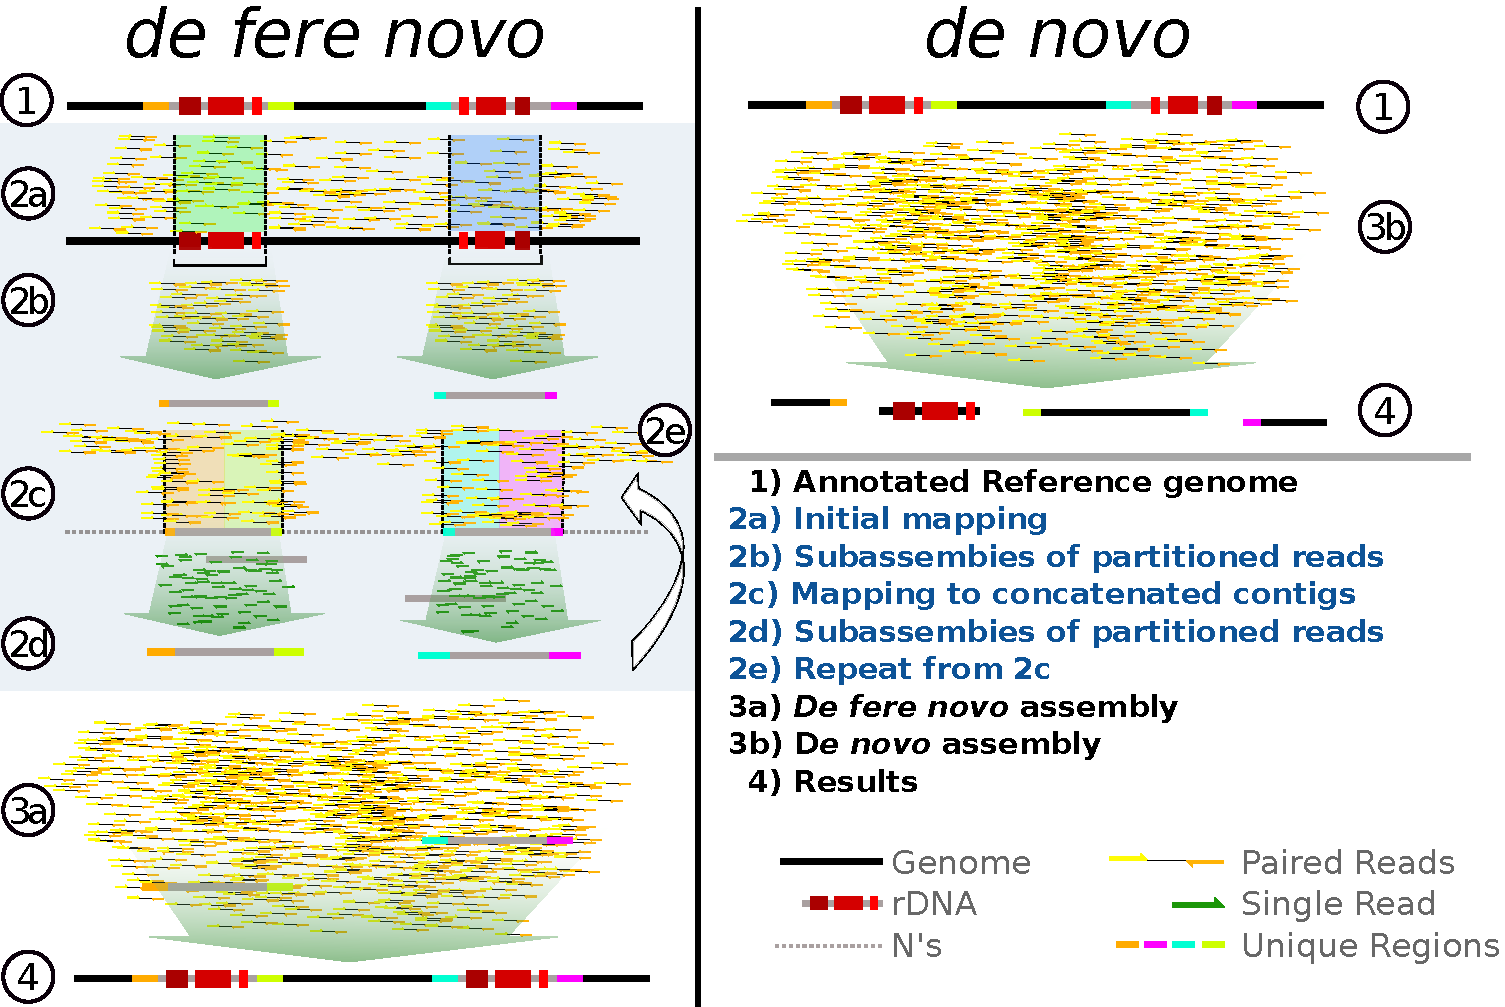
\includegraphics[width=0.75\textwidth]{riboSeed_v11}
    \caption{a nice plot}
    \label{fig:overview}
\end{figure}








%%%%%%%%%%%%%%%%%%%%%%%%%%%%%%%%%%%%%%%%%%%%%%%%%%%%
\begin{table*}
\centering
\ra{1.3}
\begin{tabular}{@{}rrrrcrrrcrrr@{}}\toprule &
\multicolumn{3}{c}{$w = 8$} & \phantom{abc} & \multicolumn{3}{c}{$w = 16$} & \phantom{abc} & \multicolumn{3}{c}{$w = 32$} \\
\cmidrule{2-4} \cmidrule{6-8} \cmidrule{10-12} &
 $t=0$ & $t=1$ & $t=2$ && $t=0$ & $t=1$ & $t=2$ && $t=0$ & $t=1$ & $t=2$\\
\midrule
$dir=1$ \\
$c$ & 0.0790 & 0.1692 & 0.2945 && 0.3670 & 0.7187 & 3.1815 && - 1.0032 & -1.7104 & -21.7969 \\
$c$ &  - 0.8651  & 50.0476& 5.9384 & & -9.0714& 297.0923& 46.2143&& 4.3590& 34.5809& 76.9167 \\
$c$ & 124.2756& - 50.9612& -14.2721&& 128.2265& -630.5455& -381.0930&& -121.0518& -137.1210& -220.2500 \\
$dir=0$ \\
$c$ & 0.0357& 1.2473& 0.2119&& 0.3593& -0.2755& 2.1764&& -1.2998& -3.8202& -1.2784 \\
$c$ & -17.9048& -37.1111& 8.8591&& -30.7381& -9.5952& -3.0000&& -11.1631& -5.7108& -15.6728 \\
$c$ & 105.5518& 232.1160&
-94.7351&& 100.2497& 141.2778& -259.7326&& 52.5745& 10.1098& -140.2130\\
\bottomrule
\end{tabular}
\caption{Caption}
\end{table*}

%%%%%%%%%%%%%%%%%%%%%%%%%%%%%%%%%%%%%%%%%%%%%%%%


\end{linenumbers}

\baselineskip13pt
\pagebreak
\bibliography{riboSeed_refs}

\end{document}
